\section{Architecture}
Для реализации системы предлагается следующий стек технологий и архитектура

\subsection{Модель архитектуры}
Система будет спроектирована на основе трёхуровневной архитектуры с применением шаблона "Layers".
Диаграмма архитектуры представлена на рис~\ref{fig:arch}.
\subsection{Стек технологий}
\begin{itemize}
	\item Frontend: реализуется с использованием React, TypeScript, и React Query
	\item Backend: Реализуется с использованием Spring Framework, Kotlin
	\item Database: В качестве системы управления базами данных используется PostgreSQL
	\item API: Взаимодействие между клиентской и серверной частями организовано через REST API. В качестве стандарта обмена данными используется формат JSON. REST API предоставляет методы для выполнения CRUD-операций и обмена данными между клиентом и сервером
	\item Авторизация и аутентификация: Аутентификация и авторизация реализуются с использованием JWT (JSON Web Token). JWT-токены используются для защиты API и передачи данных о пользователе без необходимости сохранять сеансы на сервере. Spring Security настраивается для обработки токенов и контроля доступа к защищенным ресурсам
	\item Сборка и управление зависимостями: Для сборки проекта и управления зависимостями используется Gradle, который обеспечивает гибкость и быструю интеграцию с различными плагинами и инструментами
	\item Логирование и мониторинг: Логирование реализуется с использованием Logback для записи событий и ошибок в консоль. Для удобного и структурированного логирования применяется аспектно-ориентированное программирование (AOP), которое позволяет внедрять логи в бизнес-логику без изменения самого кода, что повышает его читаемость и снижает вероятность ошибок
	\item Тестирование: Для обеспечения высокого качества кода применяются тесты с использованием JUnit, Testcontainers, Playwright. JUnit используется для написания модульных и интеграционных тестов. Testcontainers позволяют запускать тесты с реальными экземплярами сервисов (например, баз данных) в контейнерах, что обеспечивает точную симуляцию продакшн-среды для тестирования. Playwright используется для написания e2e тестов
\end{itemize}

\subsection{Диаграмма архитектуры}
\begin{figure}[h]
	\centering
	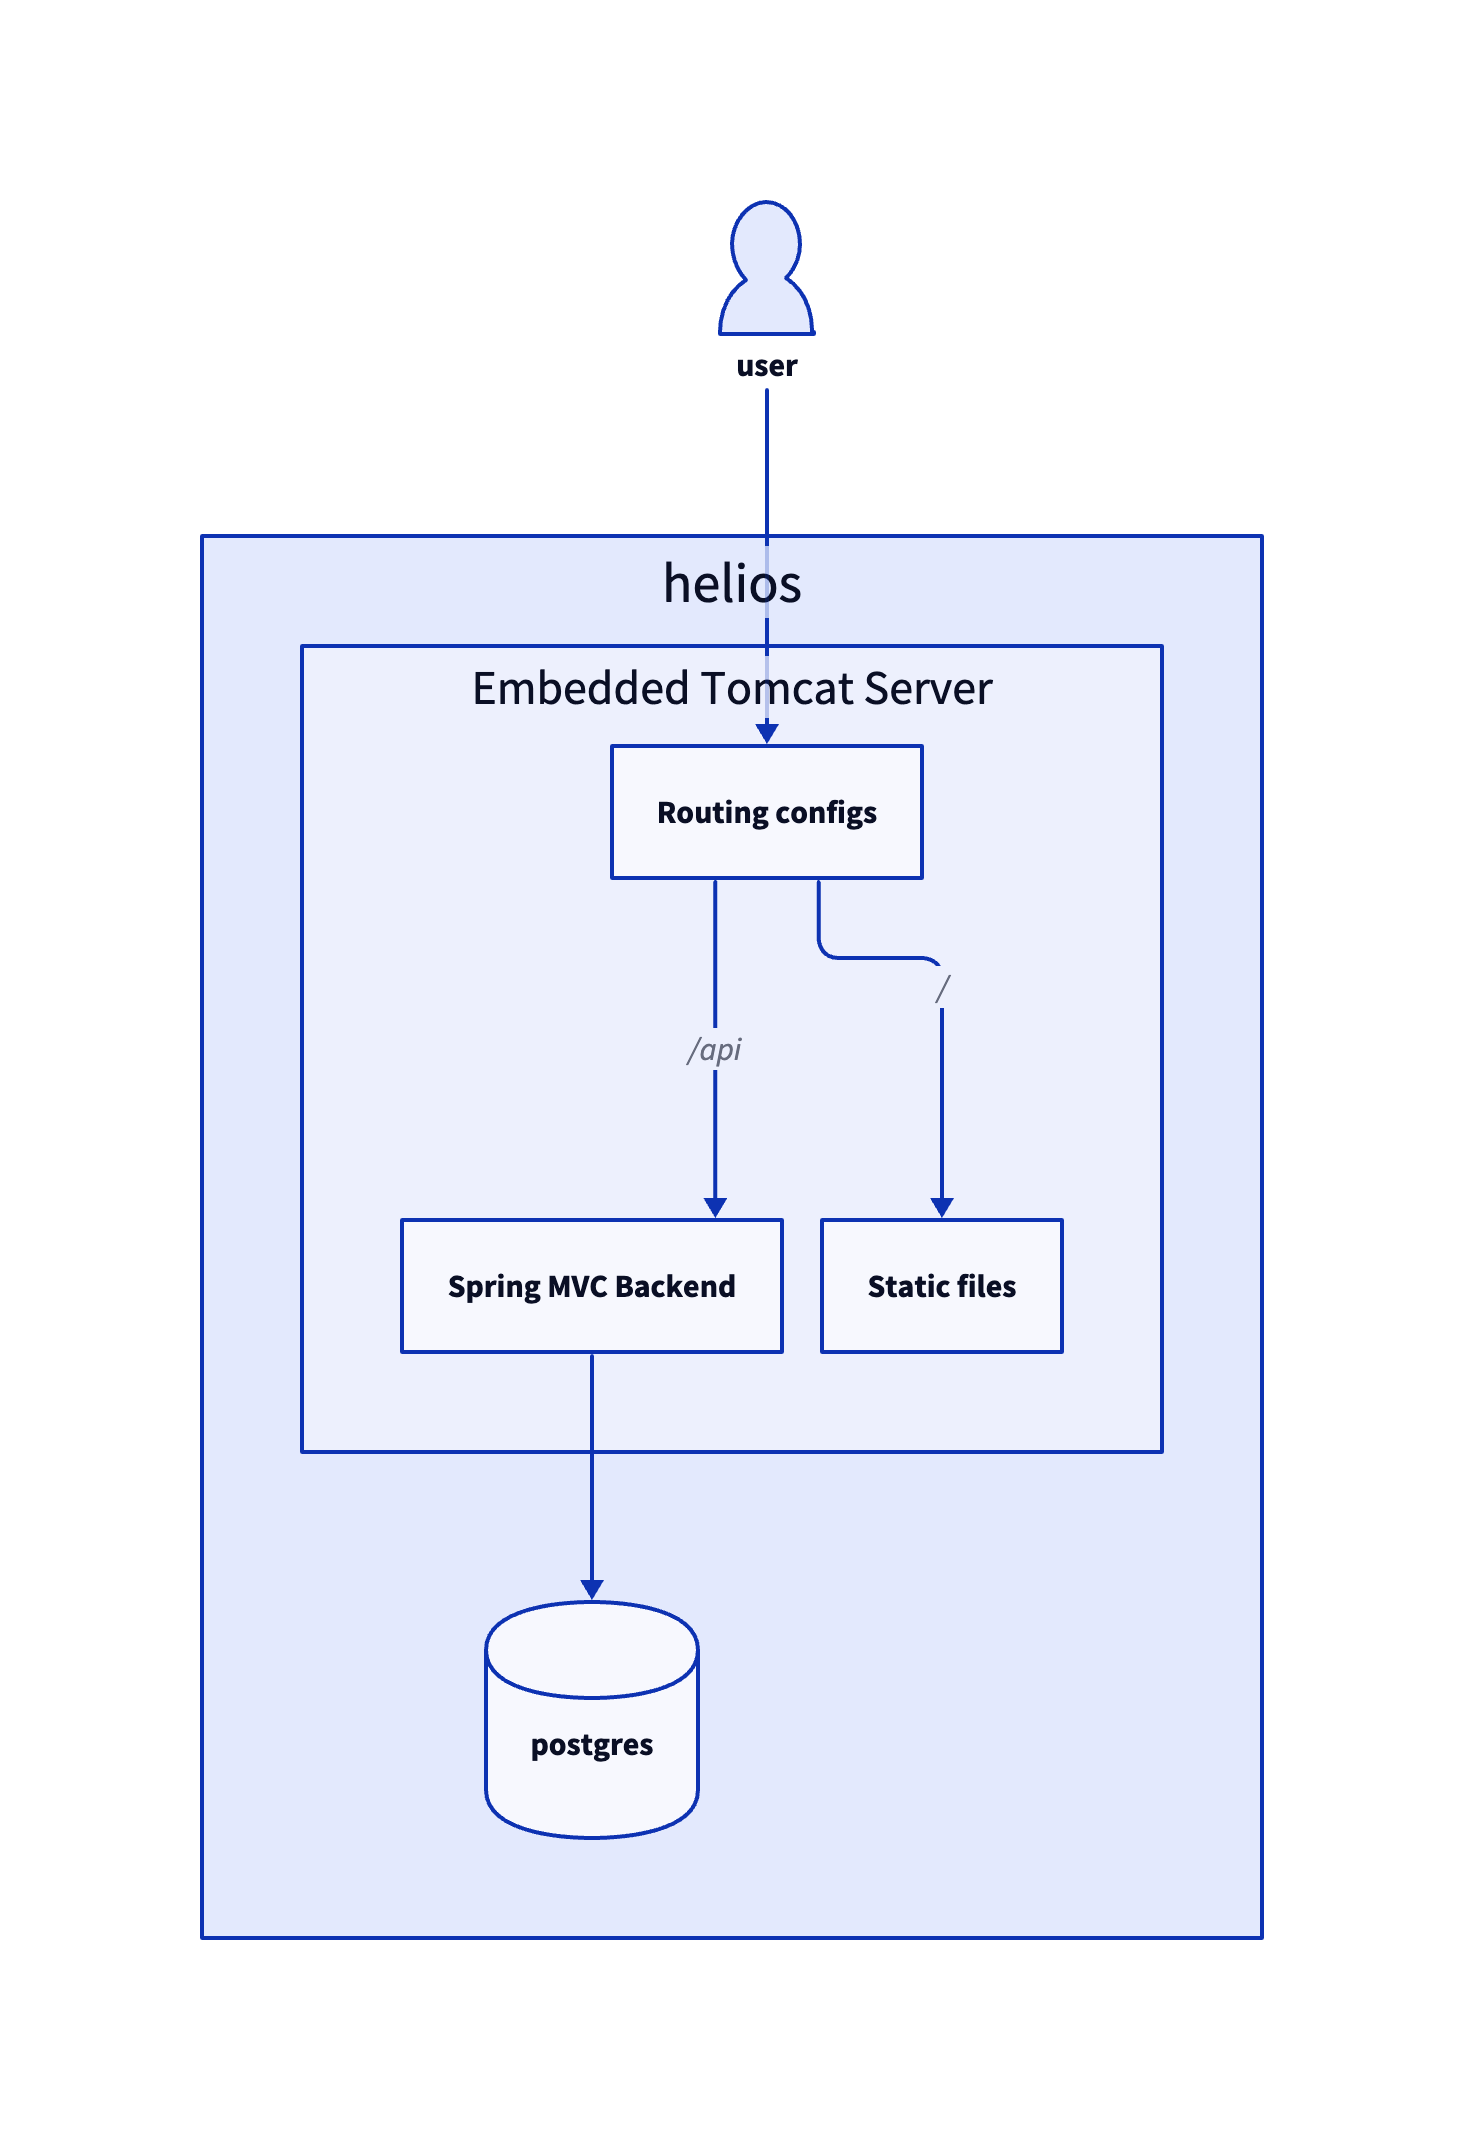
\includegraphics[width=0.5\textwidth]{./figures/architecture.png}
	\caption{Диаграмма архитектуры}\label{fig:arch}
\end{figure}
